\chapter{Acerca del documento}

\begin{quotation}
\small{
\q{\textit{Cuando eres un carpintero haciendo un mueble hermoso, no vas a usar un pedazo de mala madera para la parte trasera, pese a que esté pegada a la pared y nadie la vea. Tú sabes que está ahí. Para dormir bien por la noche, la estética, la calidad, tienen que ser llevadas hasta el final.}}
}
\end{quotation}

\begin{flushright}
\small{\textit{Steve Jobs}}
\end{flushright}

\section{Maquetación del libro}

A la hora de escribir este libro, éste ha sido desarrollado utilizando Lua\LaTeX, una versión más moderna de la familia de compiladores de \LaTeXe{}, que sustituye al conocido \textsc{pdf}\TeX{} (aunque todavía está en fase de pruebas y no es raro encontrar ciertos errores a la hora de trabajar con esta herramienta). Las ventajas que incorpora Lua\LaTeX{} son varias, por ejemplo: permite la edición de documentos en codificación \textsc{utf-8} directamente y el uso de tipografías \textsc{otf}.

Las personas que me han inspirado de alguna manera a contribuir a la maquetación final de este libro, y a las que quiero agradecer de manera particular, han sido las siguientes:

\begin{itemize}
\item Eivind Uggedal con su tesis: \work{Social Navigation on the Social Web} \cite{libro:social-navigation}.
\item Robert Bringhurst con su libro: \work{The Elements of Typographic Style} \cite{libro:bringhurst}.
\item Ellen Lupton con su libro: \work{Thinking with Type} \cite{libro:lupton}.
\end{itemize}

\section{Decisiones tipográficas}

\begin{figure}
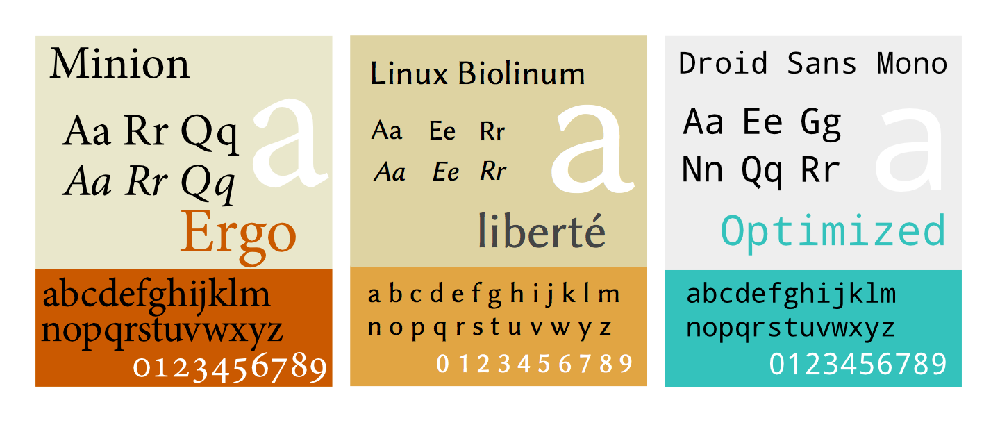
\includegraphics[width=\linewidth]{../graphics/fig_tipografias_usadas}
\caption{Muestra de las tipografías utilizadas en este libro.}
\end{figure}

El cuerpo principal de este texto está fijado a un tamaño de 12pt en una hoja \textsc{a4} y el interlineado a 15pt. Se ha utilizado la tipografía \textit{Minion Pro}, diseñada por Robert Slimbach y que está inspirada en las grafías del \textit{Renacimiento}, por ser una fuente que posee \textit{movimiento} y, a la vez, \textit{elegancia}.

Por otra parte, la tipografía elegida para listar los ejemplos se denomina \textit{Linux Biolinum} y fue creada en 2003 como una alternativa de código abierto a otras tipografías \textit{sans-serif} similares.

Por último, la tipografía usada para mostrar código fuente se denomina \textit{Droid Sans Mono}, creada por Ascender Corporation y que es utilizada en los dispositivos móviles con sistema operativo Android.

\section{Decisiones visuales}

\subsection{Ilustraciones}
Las ilustraciones empleadas al comienzo de cada capítulo (fueron elegidas por tener un significado especial para el proyecto) pertenecen a la historia \work{Jack and The Giants} (de autor desconocido) y fueron creadas por Richard Doyle en 1851. 

Podemos leer el libro de manera completamente gratuita en la siguiente dirección: \url{http://www.gutenberg.org/files/15621/15621-h/15621-h.htm}. 

\subsection{Capturas de pantalla}

Las capturas de pantalla han sido realizadas con el programa \textit{Skitch} para \textit{OS X} y que es gratuito.

\subsection{Gráficos}

Los gráficos empleados para explicar diferentes conceptos del proyecto han sido diseñados enteramente por mi utilizando el programa de dibujo vectorial \textit{OmniGraffle Pro}. He denominado a este conjunto de dibujos como: \textit{Colorful} que viene a significar del inglés como \textit{Colorido} (\figureref{ejemplo_colorful}). 

\begin{figure}
\centering
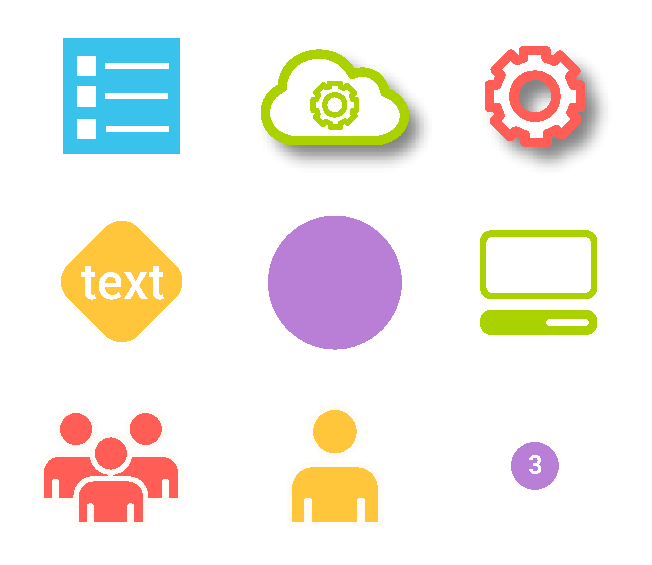
\includegraphics[width=.8\linewidth]{../graphics/fig_ejemplo_colorful}
\caption{Ejemplo de algunos de los iconos de \textit{Colorful}.}
\label{fig:ejemplo_colorful}
\end{figure}

\section{Obtención del material}

Si deseas obtener más información acerca del proyecto como: las partes más importantes de éste, como está construido el código fuente de la maquetación, el de la presentación o usar \textit{Colorful} para crear tus propios diagramas\ldots{} puedes visitar el siguiente enlace:

\begin{pyglist}[language=html]
  http://aldoborrero.com/proyectos/alma
\end{pyglist}